\documentclass[lettersize,journal]{IEEEtran}
\usepackage{amsmath,amsfonts}
\usepackage{algorithmic}
\usepackage{algorithm}
\usepackage{array}
\usepackage[caption=false,font=normalsize,labelfont=sf,textfont=sf]{subfig}
\usepackage{textcomp}
\usepackage{stfloats}
\usepackage{url}
\usepackage{verbatim}
\usepackage{graphicx}
\usepackage{cite}
\hyphenation{op-tical net-works semi-conduc-tor IEEE-Xplore}
% updated with editorial comments 8/9/2021

% \usepackage{amsmath,amsfonts}
% \usepackage{algorithmic}
% \usepackage{array}
% \usepackage[caption=false,font=normalsize,labelfont=sf,textfont=sf]{subfig}
% \usepackage{cite}
% \usepackage{textcomp}
% \usepackage{stfloats}
% \usepackage{url}
% \usepackage{verbatim}
% \usepackage{graphicx}
\usepackage{amssymb}
\usepackage{xcolor}
% \usepackage{appendix}
% \usepackage{algorithm}
\usepackage{amsthm}
% \usepackage{multirow} 
% \usepackage{multicol} 
% \usepackage{color}
\usepackage{bm}
% \hyphenation{op-tical net-works semi-conduc-tor IEEE-Xplore}
\usepackage{hyperref}
\usepackage{scalerel}
\usepackage{float}%提供float浮动环境
\usepackage{booktabs}%提供命令\toprule、\midrule、\bottomrule
\newtheoremstyle{custom}
  {\topsep}    % 上方间距
  {\topsep}    % 下方间距
  {\normalfont} % 定理内容的字体 (普通字体)
  {1em}           % 缩进量
  {\itshape}   % 定理标题的字体 (斜体)
  {:}          % 标题后的标点符号
  { }          % 标题后与内容的间距
  {\thmname{\textit{#1}}% 定理标题格式 (斜体)
   \thmnumber{ \textit{#2}}% 定理编号格式 (斜体)
   \thmnote{ \textit{(#3)}}}% 定理备注格式 (斜体)
% 应用自定义样式
\theoremstyle{custom}
\newtheorem{Thm}{Theorem}
\newtheorem{Lem}{Lemma}
\newtheorem{Cor}{Corollary}
\newtheorem{Def}{Definition}
\newtheorem{Exam}{Example}
\newtheorem{Alg}{Algorithm}
\newtheorem{Prob}{Problem}
\newtheorem{subproblem}{Problem}[Prob]
\newtheorem{Rem}{Remark}
\newcommand{\RNum}[1]{\uppercase\expandafter{\romannumeral #1\relax}}
\newcommand{\tabincell}[2]{\begin{tabular}{@{}#1@{}}#2\end{tabular}}
% \theoremseparator{:}
\newtheorem{hyp}{Hypothesis}

\begin{document}

\title{A Novel Action-Relevance-Aware Multi-View Token Allocation Approach for Wireless VLA Inference}

\author{IEEE Publication Technology,~\IEEEmembership{Staff,~IEEE,}
        % <-this % stops a space
\thanks{This paper was produced by the IEEE Publication Technology Group. They are in Piscataway, NJ.}% <-this % stops a space
\thanks{Manuscript received April 19, 2021; revised August 16, 2021.}}

% The paper headers
\markboth{Journal of \LaTeX\ Class Files,~Vol.~14, No.~8, August~2021}%
{Shell \MakeLowercase{\textit{et al.}}: A Sample Article Using IEEEtran.cls for IEEE Journals}

\IEEEpubid{0000--0000/00\$00.00~\copyright~2021 IEEE}
% Remember, if you use this you must call \IEEEpubidadjcol in the second
% column for its text to clear the IEEEpubid mark.

\maketitle

\begin{abstract}
This document describes the most common article elements and how to use the IEEEtran class with \LaTeX \ to produce files that are suitable for submission to the IEEE.  IEEEtran can produce conference, journal, and technical note (correspondence) papers with a suitable choice of class options. 
\end{abstract}

\begin{IEEEkeywords}
Article submission, IEEE, IEEEtran, journal, \LaTeX, paper, template, typesetting.
\end{IEEEkeywords}

\section{Introduction}
\IEEEPARstart{X}{xx}...  
Multi-modal sensor fusion and unstructured environment are identified as two key features of embodied AI \cite{li_developments_2025}. However, xxx. 
Wireless communication is also identified as a crucial enabling technology for embodied robotics, especially humanoid and xxx, for the flexible and ubiquitous characteristics. 

In order to fuse the multi-modal sensory data and adapt into the dynamic unstructured environments, xxx AI-assisted methods have been proposed. In the early researches, xxx. Due to its multi-task emergence abilities, VLA has become a heated research topic. \cite{}, \cite{}, \cite{} performs high-accuracy action inference in a xxx of embodied tasks. However, these architectures overlook xxx, xxx in practical deployments. 

For practical deployment, several architectures are developed to mitigate the xxx. The embodied LAM architectures are mainly divided into 2 architectures, end-to-end VLA and dual system. End-to-end VLA includes xxx, xxx, and xxx. They xxx. However the end-to-end architectures xxx and suffer latency and power consumption draw-backs on humanoid and xxx embodied systems. To mitigate these drawbacks, dual system, including Helix, InternVLA, GR00T, xxx. Although the dual system embodied AI architectures xxx, they still fail to adapt into dynamic and resource limited wireless systems. 

To fill this gap, recent token pruning methods \cite{}, \cite{} manage to xxx under single-view scenarios. \cite{}, \cite{} extend these techniques to multi-view scenarios. \cite{}, \cite{} introduce channel-quantization-sensitivity awareness and layer-sensitivity analysis, and thus manage to further reduce token overhead under computational budget limitations.  However, the above-mentioned methods fundamentally fail to theoretically derive optimal solutions under wireless scenarios. 

To fill this gap, in the area of wireless communications-enabled control systems, Wireless Netowrked Control System (WNCS) techniques \cite{}, \cite{}, \cite{} aim to optimize control performance under wireless network topologies. \cite{} derive xxx. \cite{} derive xxx. \cite{} derive xxx. However, the rigorous derivations mainly hold in linear and stationary control systems, not non-linear, unstructured embodied AI systems. Semantic-aware and goal-oriented methods \cite{}, \cite{}, \cite{} xxx. \cite{} learn a xxx-task-specific network and manage to xxx. \cite{} learn a xxx-task-specific network and manage to xxx. \cite{} learn a xxx-task-specific network and manage to xxx. However, these methods are data-hungry and require online post-adaption when task varies. Despite the corresponding performance improvements spotted in the up-mentioned methods, the fundamental performance bound for hybrid VLA data transmission under wireless links is still uninvestigated. 

\IEEEpubidadjcol
Motivated by these, our main contributions are summarized as follows: 
\begin{itemize}
    \item \textbf{Wireless-aware multi-view token allocation framework:}
    We formulate a wireless-enabled embodied AI framework in which multiple sensing nodes perform local visual-token pruning and transmit only the retained tokens to an edge VLA for action inference. 
    Different from existing VLA token-pruning methods that mainly optimize computational efficiency under fixed token budgets, we explicitly couple the per-view retained token numbers with heterogeneous wireless transmission costs and formulate the resulting action-error minimization problem under an air-interface bandwidth constraint.

    \item \textbf{Action-relevance model and delayed-feedback-aware token allocation:}
    To address the analytically intractable relationship between multi-view token pruning and nonlinear VLA action performance, we establish a calibrated marginal action-utility model that characterizes the expected action-error reduction as a function of the VLA internal action relevance and the retained token number of each view.
    Based on this model, the original action-error minimization problem is transformed into a tractable action-relevance-aware utility maximization problem.
    Moreover, considering that the VLA internal action-relevance signal is generated at the edge only after inference, we develop a causal allocation mechanism using delayed relevance feedback and derive a generalized water-filling solution that jointly accounts for task relevance, diminishing token utility, and wireless transmission cost.

    \item \textbf{Experimental validations:} xxx. 
\end{itemize}

And the rest of the paper are organized as follows. xxx. 

\section{System Model}
\begin{figure*}\label{system_model}
    \centering
    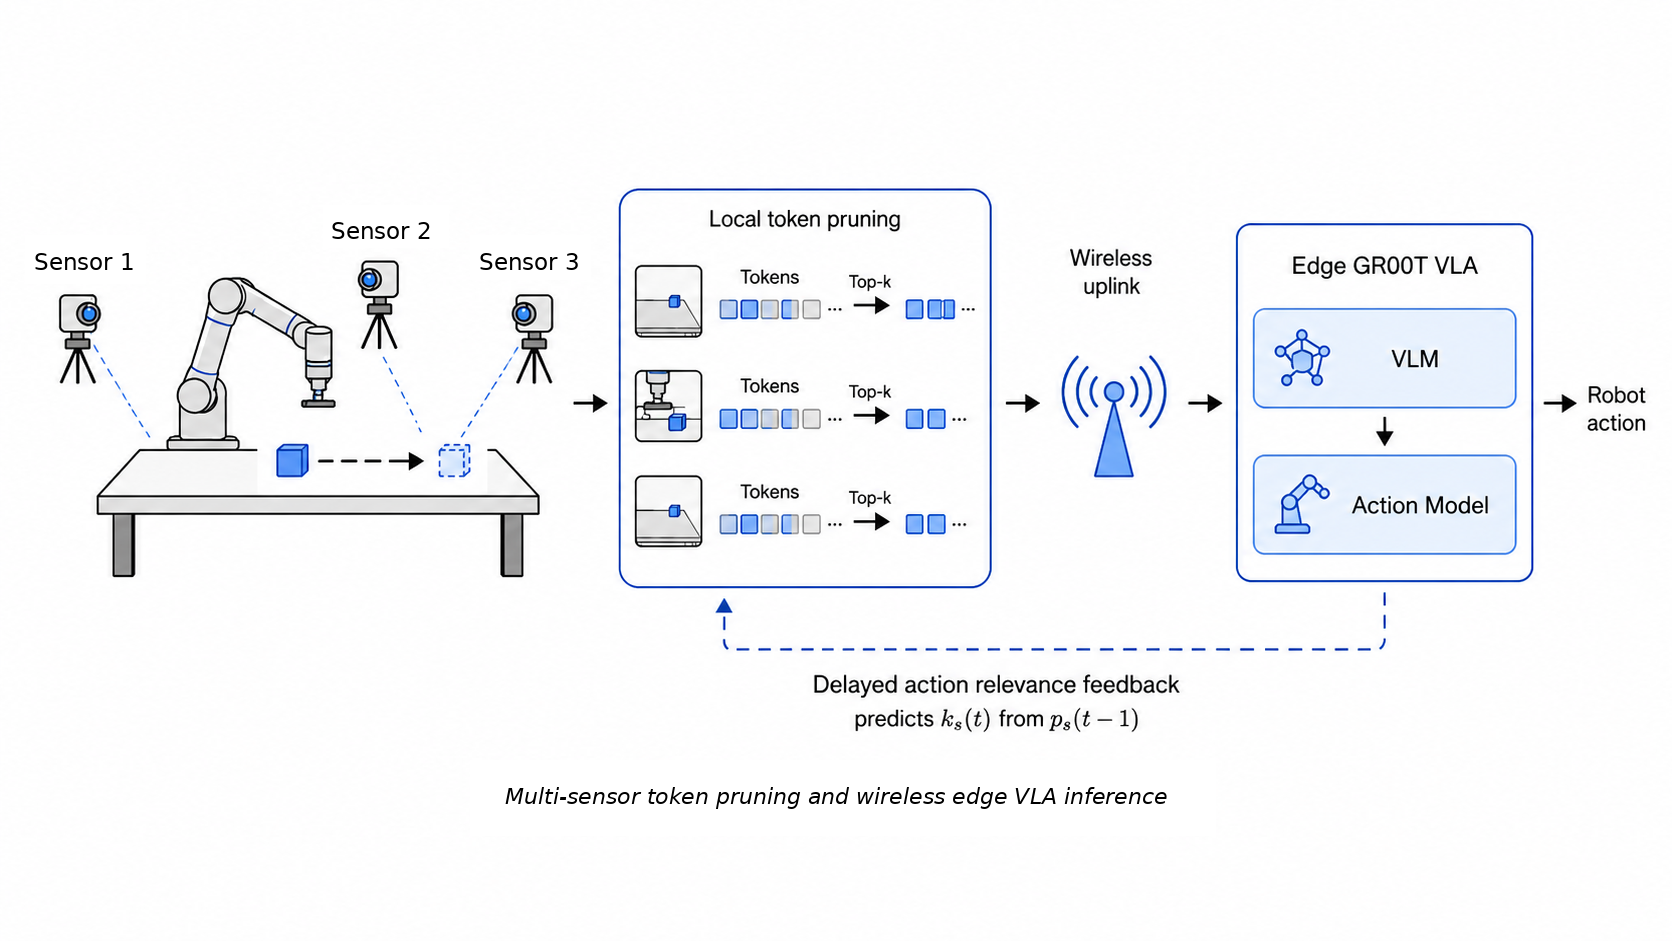
\includegraphics[width=\linewidth, trim=0 200 0 30, clip]{system_model.png}
    \caption{System model. }
    \label{fig:placeholder}
\end{figure*}
In this paper, we study a wireless-enabled embodied AI (WEEA) system, where an embodied agent and the corresponding sensing nodes $\mathcal{S} = \{1, \ldots, s, \ldots, S\}$ are connected to the edge remote controller $e$ with Vision-Language-Action (VLA) equipped. 
% $I$ agents with sensing and action abilities are distributed in the space. 
The system is illustrated in Fig.~\ref{system_model}. Each sensing node perceives the environment with observations $\mathcal{V}_s(t) \in \mathcal{V}(t)$ (e.g., RGB images), its raw data volume is identified with $d_s(t)$. The edge VLA model receive $\mathcal{V}(t)$ and a time-invariant language instruction (prompt) $p$, then VLA model generate policy $\Pi_\theta(\mathcal{A}(t) \vert \mathcal{V}(t), p)$ to predict an action sequence $\mathcal{A}(t)$ (e.g., end-effector poses or joint velocities), where $\theta$ denotes the VLA model parameter. 
% singel-cell system where the base station (BS) is equipped with edge computing power, serving a set of user equipments (UEs), denoted by $i \in \mathcal{I}$. 
% Each agent contains hybrid content transmissions of multi-modal sensory data from helper agent $j$ to ego agent $i$, denoted with ${\bf d}_{j, i}(t) = \{ d^\mathrm{v}_{j, i}(t), d^\mathrm{r}_{j, i}(t), \ldots \}$, where $d^\mathrm{v}_{j, i}(t)$, $d^\mathrm{r}_{j, i}(t)$ represent the transmission data volume of vision, radar, etc., from helper agent $j$ to ego agent $i$, respectively. 
% Each agent contains hybrid content transmissions of multi-modal sensory data and control data, profiled with ${\bf q}_i(t) = \{ {\bf q}^\mathrm{v}_i(t), {\bf q}^\mathrm{r}_i(t), {\bf q}^\mathrm{ms}_i(t), \ldots , {\bf q}^\mathrm{mc}_i(t) \}$, where ${\bf q}^\mathrm{v}_i(t) = \{ {\bf d}^\mathrm{v}_i(t), f^\mathrm{v} \}$, ${\bf q}^\mathrm{r}_i(t) = \{ {\bf d}^\mathrm{r}_i(t), f^\mathrm{r} \}$, ${\bf q}^\mathrm{ms}_i(t) = \{ d^\mathrm{ms}_i(t), f^\mathrm{ms} \}$ and ${\bf q}^\mathrm{mc}_i(t) = \{ d^\mathrm{mc}_i(t), f^\mathrm{mc} \}$ represent the transmission profile of vision, radar, motor state and motor control for agent $i$, including data volume and transmission frequency, respectively. 


% \subsection{xxx Protocol Design}
% Identifying the multi-modal sensory feedback

% The communication resource grid is 



% Puncturing\footnote{xxx} and finite block-length short packet transmission are enabled for ultra low-latency high-reliability motor state and control signal transmissions. The puncturing duration at sub-channel $f$ is denoted by $t_{i, f} < T_k, i \in \mathcal{I}_{m}$. 
% % Puncturing\footnote{xxx} is enabled for ultra low-latency high-reliability transmissions, which is suitable for text queries transmissions carrying more semantic information within each bits \cite{}. 

\subsection{Communication Model}
The up-link transmission rate from sensing node $s$ to the edge server at slot $t$ is described as
\begin{align}
    r_{s}(t) = B_s(t) log_2\left(1 + \mathrm{SNR}_s(t) \right), \forall s \in \mathcal{S}, 
\end{align}
where $B_s(t)$ and $\mathrm{SNR}_s(t)$ denote the fractional bandwidth allocated to $s$ and the signal-to-noise ratio (SNR) of $s$, respectively. The fractional bandwidth allocation follows
\begin{align}\label{bandwidth_cons}
    \sum_{s \in \mathcal{S}}B_s(t) \leq B, 
\end{align}
where $B$ is the system bandwidth\footnote{We assume that adequate bandwidth $B$ is semi-persistently allocated to the WEEA system via orthogonal radio access network (RAN) slicing techniques \cite{}, \cite{}}. 

% The transmission rate from helper agent $j$ to ego agent $i$ at slot $t$ is described as: 
% \begin{align}
%     r_{j, i}(t, f) = B \sum_{f \in \mathcal{F}} b_{f, j, i}(t) \log_2\left(1 + \frac{p_{j, i}(t) h_{j, i}(t)}{\vartheta^2} \right), 
%     % i \in \mathcal{I}_i \cup \mathcal{I}_v &, 
% \end{align}
% % \begin{align}
% %     r_{n, i}(t, f) = (1 - \sum_{i \in \mathcal{I}_\mathrm{t}}\frac{t_{i, f}}{T_k})\log_2\left(1 + \frac{p_{n, i}(t) h_{n, i}(t)}{\vartheta^2} \right) &, \nonumber\\
% %     i \in \mathcal{I}_i \cup \mathcal{I}_v &, 
% % \end{align}
% where $h_{j, i}(t)$ is the channel coefficient from $j$ to $i$, $B$ is unit bandwidth of sub-channel, $\vartheta$ is the xxx and $b_{f, j, i}(t)$, $p_{j, i}(t)$ is the sub-channel allocation indicator and the transmit power, respectively. $b_{f, j, i}(t) = 1$ means sub-channel $f$ is allocated for the data transmission from $j$ to $i$ and $b_{f, j, i}(t) = 0$ otherwise.  The transmit power of each agent $i$ is bounded by 
% \begin{align}
%     \sum_{i \in \mathcal{I}, i \neq j} p_{j, i}(t) \leq P_\mathrm{max}. 
% \end{align}
% Transmission power consumption \cite{xu_energy-efficient_2013} for each BS $n$ is given as
% \begin{align}
%     P_{n}^{\mathrm{com}} = P_S + \alpha \cdot P_T
% \end{align}
% where $P_S$ and $\alpha$ represents the static circuit power and the power amplification coefficient, respectively. 

\subsection{Top-$k$-enabled Token Compression Model}
% Each edge server cache a set of $\mathcal{L}_n$ LAMs. 
In order to support timely and efficient perceptional data delivery, top-$k$ Token compression techniques are widely investigated \cite{}, \cite{}. 

Through Tokenization and top-$k$ Token pruning, the raw observations $\mathcal{V}_s(t)$ are locally compressed at $s$ in terms of observation feature\footnote{On-device/local Tokenizers and Token pruning Techniques are proved to be applicable and helpful in the area of multi-view VLA systems \cite{}, \cite{}. }, and thus we have the exact air-interface transmission data volume denoted as: 
\begin{align}
    d_s^{k_s(t)}(t) = \frac{\alpha_s k_s(t)}{n_s} d_s(t), \forall s \in \mathcal{S}, 
\end{align}
where $\alpha_s$, $k_s(t)$ and $n_s$ denote the normalized xxx rate for the LAM Tokenizer, the output Token length after top-$k$ token pruning and the original Token length, respectively. We denote the slot-$t$ top-$k$ decision vector as ${\bf k}(t)=\{k_1(t),\ldots,k_S(t)\}$ and the complete decision sequence as ${\bf k}=\{{\bf k}(t)\}_{t=1}^{T}$. $k_s(t)$ follows
\begin{align}\label{token_cons}
    k_s^{\min}\leq k_s(t)\leq n_s,\quad k_s(t)\in\mathbb Z_+, \ \forall s,
\end{align}
where $k_s^{\min}$ denotes the minimum Token number of sensor $s$. 

With top-$k$ Token compression, the corresponding VLA model in the WEEA system suffers the performance degradation, and the comprehensive VLA output performance in terms of long-term average action mean square error (MSE) \cite{} is denoted by 
\begin{align}
    \epsilon_{\bf k} = \mathbb{E} \left[\sum_{t = 1}^T\vert\vert \mathcal{A}_{\bf k}(\mathcal{V}(t)) - \mathcal{A}^*(\mathcal{V}(t)) \vert\vert^2_2\right], 
\end{align}
where $\mathcal{A}_{\bf k}(\mathcal{V}(t))$ is the action generated with the pruned multi-view observations and $\mathcal{A}^*(\mathcal{V}(t))$ is the reference action, e.g., the action generated by the full-token VLA during calibration or an expert action when available. 

% The transmission data volume from helper agent $j$ to ego agent $i$ with top-$k$ Token pruning \cite{} is given by 
% \begin{align}
%     d^\mathrm{v}_{j, i}(t) = \frac{k^\mathrm{v}_{j, i}}{n^\mathrm{v}}D^\mathrm{v}_{j, i}(t), 
% \end{align}
% % where xxx. And the corresponding QoS metrics for each LAM in terms of accuracy and delay are listed as follows
% where ${\bf k} = \{ \{k^\mathrm{v}_{j, i}\}, \{k^\mathrm{r}_{j, i}\}, \ldots \}$ denotes the whole set of top-$k$ Token pruning rate. 

% And the corresponding VLA inference action error requirement of agent $i$ is listed as follows
% \begin{align}\label{accuracy_cons}
%     \epsilon_i({\bf k}, t) \leq \delta_i, \forall i \in \mathcal{I}, 
% \end{align}
% % \begin{align}\label{accuracy_delay_cons}
% % \left\{
% %     \begin{array}{l l}
% %         q() \geq \rho_l, \forall l \in \mathcal{L}_n, \forall n \in \mathcal{N}_{BS}, \\
% %         d() \leq \delta_l, \forall l \in \mathcal{L}_n, \forall n \in \mathcal{N}_{BS}. 
% %     \end{array}
% % \right. 
% % \end{align}
% where $\epsilon_i({\bf k})$ and $\delta_i$ denotes the VLA inference error and error threshold of agent $i$, respectively. 
% % where $\rho_l$ and $\delta_l$ are corresponding accuracy and delay thresholds of LAM $l$. 

% Computing power consumption for each agent $i$ is given according to the well investigated dynamic voltage and frequency scaling (DVFS) \cite{guerreiro_modeling_2019} as follows
% \begin{align}
%     P_{i}^{\mathrm{comp}} = 
% \end{align}

\section{Problem Formulation}
We have the original action error minimization problem given by
\begin{Prob}[Original Action Error Minimization Problem]\label{prob:p1}
    The action error of the WEEA system can be minimized via
    \begin{align}
        \underset{\{{\bf k}(t)\},\{B_s(t)\}}{\textrm{minimize}} \quad & \epsilon_{\bf k} \nonumber\\
        \textrm{subject to} \quad
        & \tau r_s(t) \geq d_s^{k_s(t)}(t), \ \forall s, \label{rate_cons}\\
        % & \sum_{s\in\mathcal S}B_s(t)\leq B, \ \forall t, \nonumber\\
        & \eqref{bandwidth_cons}, \eqref{token_cons}, \nonumber
    \end{align}
    where $\tau$ is the transmission duration of one control slot. Constraint \eqref{rate_cons} guarantees that all retained visual tokens can be delivered to the edge within the current slot.
\end{Prob}

Problem~\ref{prob:p1} is difficult because the action error $\epsilon_{\bf k}$ is induced by the nonlinear VLA inference pipeline and has no explicit analytical form with respect to the retained token numbers. Moreover, different camera views have heterogeneous action relevance and different marginal redundancy as the retained token number increases. Finally, the action-relevance signal is generated at the edge only after VLA inference, and hence it is available to the sensing nodes with at least one-slot feedback delay.

\section{Problem Transformation}
\subsection{Equivalent Communication-Cost Reformulation}
By substituting the rate and token-volume models into \eqref{rate_cons}, the minimum bandwidth required by sensing node $s$ at slot $t$ is
\begin{align}
    B_s(t) \geq c_s(t) k_s(t),
\end{align}
where the bandwidth cost of retaining one token is
\begin{align}\label{eq:token_cost}
    c_s(t) \triangleq
    \frac{\alpha_s d_s(t)}{n_s\tau\log_2\!\left(1+\mathrm{SNR}_s(t)\right)}.
\end{align}
Therefore, the existence of a feasible bandwidth allocation $\{B_s(t)\}$ is equivalent to
\begin{align}\label{eq:reduced_bandwidth}
    \sum_{s\in\mathcal S}c_s(t)k_s(t)\leq B.
\end{align}
Thus, the communication variables $\{B_s(t)\}$ can be eliminated without approximation.

\subsection{Action-Relevance Feedback}
After receiving the pruned multi-view visual tokens, the edge VLA generates the control action and an internal action-conditioned relevance score for each view. Let $p_s(t)\geq0$ denote the normalized relevance of view $s$, with $\sum_s p_s(t)=1$. In practice, $p_s(t)$ can be obtained by aggregating the action-to-visual internal contribution (e.g., cross-attention weighted visual values) over all retained tokens belonging to view $s$.

Since $p_s(t)$ is available only after slot-$t$ inference, it cannot causally determine $k_s(t)$. We therefore use the most recent feedback to construct a one-step prediction
\begin{align}\label{eq:relevance_predictor}
    \widetilde p_s(t)
    =\left[p_s(t-1)+\rho\big(p_s(t-1)-p_s(t-2)\big)\right]^+,
\end{align}
followed by normalization
\begin{align}
    \widehat p_s(t)=\frac{\widetilde p_s(t)}{\sum_{j\in\mathcal S}\widetilde p_j(t)+\varepsilon_p},
\end{align}
where $\rho\in[0,1]$ controls the temporal extrapolation and $\varepsilon_p$ is a small positive constant. The special case $\rho=0$ corresponds to directly using the one-slot-delayed relevance.

\begin{Lem}[Calibrated approximate transformation]\label{lem:marginal_law}
For a fixed target dataset $\mathcal D$ satisfying the calibration conditions specified in Appendix~\ref{app:calibration}, there exist camera-specific constants $\beta_s>0$ and $\gamma_s>0$ such that
\begin{align}\label{eq:marginal_law}
    \mathbb E_{\mathcal D}\!\left[
    -\frac{\Delta\epsilon_{\bf k}}{\Delta k_s}
    \Bigm| p_s,k_s\right]
    \simeq
    \beta_s\frac{p_s}{(k_s+1)^{\gamma_s}}.
\end{align}
Accordingly, define
\begin{align}\label{eq:utility}
U_s(k_s;p_s)=
\begin{cases}
\displaystyle
\frac{\beta_s p_s}{1-\gamma_s}
\left[(k_s+1)^{1-\gamma_s}-1\right], & \gamma_s\neq1,\\[2mm]
\displaystyle
\beta_s p_s\log(k_s+1), & \gamma_s=1.
\end{cases}
\end{align}
Then the dataset-averaged action error satisfies
\begin{align}\label{eq:error_surrogate}
    \mathbb E_{\mathcal D}[\epsilon_{\bf k}\mid{\bf p}]
    \simeq C({\bf p})-\sum_{s\in\mathcal S}U_s(k_s;p_s),
\end{align}
where $C({\bf p})$ is independent of ${\bf k}$. Hence, after the exact communication-cost reformulation in \eqref{eq:reduced_bandwidth}, Problem~\ref{prob:p1} is approximately equivalent, in the dataset-averaged sense, to maximizing the sum utility in \eqref{eq:utility}. The calibration, fitted parameters, validation results, and justification of this approximation are given in Appendix~\ref{app:calibration}.
\end{Lem}

Using the causal relevance prediction $\widehat p_s(t)$, we obtain the tractable per-slot surrogate problem
\begin{Prob}[Action-Relevance-Aware Token Allocation]\label{prob:p2}
\begin{align}
    \underset{\{k_s(t)\}}{\textrm{maximize}}\quad
    & \sum_{s\in\mathcal S}U_s\!\left(k_s(t);\widehat p_s(t)\right) \label{eq:p2obj}\\
    \textrm{subject to}\quad
    & \sum_{s\in\mathcal S}c_s(t)k_s(t)\leq B, \nonumber\\
    & k_s^{\min}\leq k_s(t)\leq n_s,\quad k_s(t)\in\mathbb Z_+,\ \forall s. \nonumber
\end{align}
\end{Prob}
Problem~\ref{prob:p2} preserves three key effects: a larger predicted action relevance $\widehat p_s(t)$ increases the token budget of view $s$, a larger wireless token cost $c_s(t)$ discourages its transmission, and a larger $\gamma_s$ causes the marginal benefit of additional tokens to decay faster.

\section{Proposed Solutions}
\subsection{Continuous Relaxation and Generalized Water Filling}
We first relax $k_s(t)$ to a continuous variable. Since $U_s(k_s;\widehat p_s)$ is concave for $\gamma_s>0$ and the bandwidth constraint is affine, the relaxed Problem~\ref{prob:p2} is a convex optimization problem after sign reversal. Let $\lambda(t)\geq0$ be the multiplier associated with \eqref{eq:reduced_bandwidth}. For an interior solution, the KKT condition gives
\begin{align}
    \frac{\beta_s\widehat p_s(t)}{(k_s(t)+1)^{\gamma_s}}
    =\lambda(t)c_s(t).
\end{align}
Hence, the continuous optimal token number is
\begin{align}\label{eq:waterfill}
    k_s^{\rm c}(t)
    =\left[
    \left(
    \frac{\beta_s\widehat p_s(t)}{\lambda^\star(t)c_s(t)}
    \right)^{\!1/\gamma_s}-1
    \right]_{k_s^{\min}}^{n_s},
\end{align}
where $[x]_a^b\triangleq\min\{b,\max\{a,x\}\}$ and $\lambda^\star(t)$ is selected such that the bandwidth constraint is met. Since $\sum_s c_s(t)k_s^{\rm c}(t)$ is monotonically non-increasing in $\lambda$, $\lambda^\star(t)$ can be obtained efficiently by bisection.

\subsection{Integer Token Allocation and Local Pruning}
The continuous solution is converted to an integer feasible solution by first setting
\begin{align}
    k_s(t)=\left\lfloor k_s^{\rm c}(t)\right\rfloor,
\end{align}
and then greedily assigning the remaining bandwidth to the camera with the largest marginal utility per unit bandwidth,
\begin{align}\label{eq:greedy_index}
    \Psi_s(t)=
    \frac{\beta_s\widehat p_s(t)}{c_s(t)(k_s(t)+1)^{\gamma_s}},
\end{align}
while maintaining \eqref{eq:reduced_bandwidth}. Once $k_s(t)$ is determined, sensing node $s$ retains its locally highest-ranked $k_s(t)$ visual tokens according to the adopted top-$k$ token-pruning score and transmits only those tokens to the edge VLA. The edge performs VLA inference, executes the action, extracts $p_s(t)$ from its internal action-conditioned signal, and feeds the compact view-level relevance vector back for slot $t+1$.

\begin{algorithm}[t]
\caption{Delayed Action-Relevance-Aware Token Allocation}\label{alg:allocation}
\begin{algorithmic}[1]
\REQUIRE Dataset-calibrated $\{\beta_s,\gamma_s\}_{s\in\mathcal S}$; $B$; $k_s^{\min}$; previous feedback $p_s(t-1),p_s(t-2)$.
\STATE Each sensing node obtains $d_s(t)$ and the current channel state; compute $c_s(t)$ using \eqref{eq:token_cost}.
\STATE Predict $\widehat p_s(t)$ using \eqref{eq:relevance_predictor} and normalize over all views.
\STATE Find $\lambda^\star(t)$ by bisection and compute $k_s^{\rm c}(t)$ using \eqref{eq:waterfill}.
\STATE Set $k_s(t)\leftarrow\lfloor k_s^{\rm c}(t)\rfloor$ for all $s$.
\WHILE{the residual bandwidth can accommodate at least one additional token}
    \STATE Compute $\Psi_s(t)$ in \eqref{eq:greedy_index} for all feasible cameras.
    \STATE $s^\star\leftarrow\arg\max_s\Psi_s(t)$ and $k_{s^\star}(t)\leftarrow k_{s^\star}(t)+1$.
\ENDWHILE
\STATE Each camera locally keeps its top-$k_s(t)$ visual tokens and transmits them to the edge.
\STATE The edge VLA infers the action, extracts $p_s(t)$, and feeds $\{p_s(t)\}$ back for the next slot.
\end{algorithmic}
\end{algorithm}

\section{Performance Analysis}
\subsection{Interpretation of the Allocation Rule}
Equation \eqref{eq:waterfill} explicitly couples embodied-task relevance and wireless cost. A camera with larger $\beta_s\widehat p_s(t)$ receives more tokens because its retained visual information yields a larger expected action-error reduction, whereas a camera with a larger $c_s(t)$ receives fewer tokens because each retained token consumes more bandwidth. The exponent $\gamma_s$ controls how quickly a view saturates: a larger $\gamma_s$ produces a faster marginal-utility decay and therefore prevents excessive token concentration on that view.

\subsection{Computational Complexity}
For a bisection tolerance $\delta_\lambda$, finding $\lambda^\star(t)$ requires $\mathcal O(S\log(1/\delta_\lambda))$ arithmetic operations. The integer correction requires at most a small number of residual-token assignments after flooring. Local top-$k$ selection can be implemented in $\mathcal O(n_s\log k_s)$ time using a heap, and all expensive VLA inference remains at the edge. Therefore, the online resource-allocation overhead is negligible compared with VLA inference.

\section{Simulation Results}

\subsection{Experimental Setup}

We evaluate the proposed method on the RoboCasa benchmark
\cite{robocasa2024} using the GR00T-N1.6-3B VLA model
\cite{nvidia_gr00t_2025}. We focus on the
\emph{PnPSinkToCounter} task, which contains 300 recorded
trajectories. Among them, 75 episodes are used for offline calibration
of the camera-specific marginal-utility parameters, while another
disjoint set of 75 episodes is used for testing. Ten temporally uniform
states are sampled from each selected episode. Each observation contains
three synchronized RGB views, denoted by \emph{side0}, \emph{side1},
and \emph{wrist0}. Each view is represented by a $9\times9$ grid of
81 visual tokens, and at least eight tokens are retained to maintain
minimum visual coverage.

The native sampling frequency of the dataset is 20 Hz; hence, the
transmission duration of one control slot is set to $\tau=50$~ms.
The total uplink bandwidth is set to $B=20$~MHz. To convert the normalized communication model used in our evaluation
into physical units, we note that all camera observations use the same
resolution and tokenization configuration. We therefore approximate
the full-token payload $d_s(t)$ as constant across time and camera
views and denote it by $d_s$. We set $\alpha_s=1$ and use an equivalent
full-token payload of $d_s=2.283$~Mbit per view. Accordingly,
$\alpha_s d_s/(n_s\tau)=0.5637$~Mbit/s. At the reference mean SNR
levels, transmitting all 243 visual tokens (81 tokens per view)
requires approximately 40~MHz of bandwidth; hence, the adopted
$B=20$~MHz budget represents a 50\% bandwidth reduction relative to
full-token transmission.

Let $\Gamma_s(t)=10\log_{10}\mathrm{SNR}_s(t)$ denote the SNR in dB.
The time-varying channel is generated using a first-order Gauss--Markov
process,
\begin{align}
\Gamma_s(t)
={}&\mu_s+\rho_c\bigl(\Gamma_s(t-1)-\mu_s\bigr)
\nonumber\\
&+\sigma_{\Gamma}\sqrt{1-\rho_c^2}\,z_s(t),
\label{eq:simulation_channel}
\end{align}
where $z_s(t)\sim\mathcal{N}(0,1)$, $\rho_c=0.9$, and
$\sigma_{\Gamma}^2 = 9$~dB. Before clipping, its stationary marginal
distribution is therefore
$\mathcal{N}(\mu_s,9~\mathrm{dB}^2)$. The camera-specific mean is
$\mu_s=\bar{\Gamma}+\delta_s$, where the offsets for
(\emph{side0}, \emph{side1}, \emph{wrist0}) are
$(-1.5,0,1.5)$~dB. We use $\bar{\Gamma}=10$~dB for the convergence
and dynamic-allocation evaluations. For the baseline comparison,
$\bar{\Gamma}$ is varied from 12 to 20~dB in steps of 2~dB.

The performance metric is the normalized action MSE between the action
chunk generated from the pruned visual tokens and the full-token action
chunk at the same robot state. A lower MSE indicates better preservation
of the original VLA action. We compare the proposed method with a
communication-only BestCQI scheme and a random feasible-$k$ scheme.
BestCQI first guarantees $k_s^{\min}$ tokens for each view and allocates
the residual bandwidth in descending order of instantaneous CQI,
without using action relevance. The random scheme starts from the same
minimum allocation and randomly assigns additional feasible tokens.
All methods use identical robot states, channel realizations, bandwidth
budgets, full-token reference actions, and diffusion seeds. The
baseline results are averaged over 225 paired inference states per SNR
point, and the 95\% confidence intervals are obtained using 5,000
episode-level bootstrap resamples. All experiments
are performed on a single NVIDIA GeForce RTX 4090 GPU.

\begin{table*}[t]
\caption{VLA and Wireless Simulation Parameters}
\label{tab:simulation_parameters}
\centering
\footnotesize
\renewcommand{\arraystretch}{1.12}
\setlength{\tabcolsep}{5pt}
\begin{tabular}{
    p{0.13\textwidth}
    p{0.12\textwidth}
    p{0.45\textwidth}
    p{0.20\textwidth}}
\toprule
\textbf{Category} &
\textbf{Symbol} &
\textbf{Definition} &
\textbf{Value} \\
\midrule

System
& $S$
& Number of camera views
& $3$ \\

& $\tau$
& Transmission duration of one control slot
& $50$ ms \\

& $B$
& Total uplink bandwidth
& $20$ MHz \\

& $d_s$
& Equivalent full-token payload per camera view
& $2.283$ Mbit \\

& $\alpha_s$
& Tokenization data-volume scaling factor
& $1$ \\

\midrule

Token pruning
& $n_s$
& Original number of visual tokens per view
& $81$ \\

& $k_s^{\min}$
& Minimum retained tokens per view
& $8$ \\

& $\mathcal{K}_s$
& Token grid used for marginal-utility calibration
& $\{8,24,48,72,81\}$ \\

\midrule

Wireless channel
& $\bar{\Gamma}$
& Reference mean SNR for convergence and dynamic allocation
& $10$ dB \\

& $\boldsymbol{\delta}$
& Mean-SNR offsets for
(\emph{side0}, \emph{side1}, \emph{wrist0})
& $(-1.5,0,1.5)$ dB \\

& $\sigma_{\Gamma}^{2}$
& SNR variance
& $9~\mathrm{dB}^{2}$ \\

& $\rho_c$
& Temporal channel correlation coefficient
& $0.9$ \\

\midrule

Allocation
& $\rho$
& Delayed-relevance prediction coefficient
& $0.25$ \\

& $\varepsilon_p$
& Relevance-normalization constant
& $10^{-8}$ \\

& $\boldsymbol{\beta}$
& Sensitivity coefficients ordered as
(\emph{side0}, \emph{side1}, \emph{wrist0})
& $(0.005788,0.01925,0.6597)$ \\

& $\boldsymbol{\gamma}$
& Power-law exponents ordered as
(\emph{side0}, \emph{side1}, \emph{wrist0})
& $(1.333,1.623,2.322)$ \\

& $I_{\max}$
& Maximum number of bisection iterations
& $200$ \\

& $\delta_{\lambda}$
& Normalized bisection tolerance
& $10^{-9}$ \\

\bottomrule
\end{tabular}
\end{table*}

The quantities $p_s(t)$, $\widehat p_s(t)$, $c_s(t)$, $k_s(t)$,
$B_s(t)$, and $\lambda^\star(t)$ are not fixed simulation parameters.
They are measured, predicted, or optimized independently at every
inference slot according to the instantaneous observation and channel
state.
 
\section{Conclusions}

\appendices
\section{Offline Calibration of the Camera-Specific Marginal Utility Law}\label{app:calibration}
This appendix describes how the dataset-level parameters $\{\beta_s,\gamma_s\}$ in Lemma~\ref{lem:marginal_law} are obtained. The calibration is performed once before deployment and does not introduce online optimization or model training.

\subsection{Calibration Assumptions}
The calibration is valid for a target dataset $\mathcal D$ under the following conditions: (i) the number, identity, intrinsics, extrinsics, and nominal placement of all cameras are unchanged between calibration and deployment; (ii) the same VLA checkpoint, visual tokenizer, token-pruning mechanism, and action normalization are used; (iii) calibration and deployment episodes are sampled from the same task/data distribution; and (iv) the tested token range covers the token budgets expected during deployment. If these conditions are violated, $\beta_s$ and $\gamma_s$ should be recalibrated.

\subsection{Counterfactual Marginal-Gain Sampling}
Let $\mathcal D_{\rm cal}\subset\mathcal D$ be a calibration subset that is disjoint from the final test episodes. For a sampled state $z$ and camera $s$, we first perform a reference full-token VLA forward pass to obtain the view relevance $p_s(z)$. This relevance is frozen during the following counterfactual sweep. We then vary only the retained token number of camera $s$ over a predefined grid $\mathcal K_s=\{k_{s,1},\ldots,k_{s,L}\}$ while keeping the other experimental settings fixed. For two adjacent token numbers, define the finite-difference marginal action gain as
\begin{align}\label{eq:cal_marginal}
    y_{s,i}(z)
    =\frac{\epsilon_{s,k_{s,i}}(z)-\epsilon_{s,k_{s,i+1}}(z)}
    {k_{s,i+1}-k_{s,i}},
\end{align}
which approximates $-\Delta\epsilon/\Delta k_s$. The action error is computed using the same reference-action definition as in Problem~\ref{prob:p1}. To suppress state-dependent VLA noise, samples are grouped into calibration-defined bins and the bin-wise expected marginal gain is used for fitting.

\subsection{Parameter Estimation}
For camera $s$, the calibration model is
\begin{align}\label{eq:cal_fit}
    \bar y_{s,i}
    =\beta_s\frac{\bar p_{s,i}}{(\bar k_{s,i}+1)^{\gamma_s}}+\xi_{s,i},
\end{align}
where $\xi_{s,i}$ is the residual. We estimate the camera-specific parameters by nonlinear least squares,
\begin{align}\label{eq:cal_nls}
    (\beta_s^\star,\gamma_s^\star)
    =\arg\min_{\beta_s>0,\gamma_s>0}
    \sum_i w_{s,i}
    \left(
    \bar y_{s,i}-
    \beta_s\frac{\bar p_{s,i}}{(\bar k_{s,i}+1)^{\gamma_s}}
    \right)^2,
\end{align}
where $w_{s,i}$ can be chosen as the number of samples in each bin or the inverse estimated variance of the bin mean. For any fixed $\gamma_s$, $\beta_s$ has the closed-form weighted least-squares solution
\begin{align}\label{eq:beta_closed}
    \beta_s^\star(\gamma_s)
    =\frac{\sum_i w_{s,i}x_{s,i}(\gamma_s)\bar y_{s,i}}
    {\sum_i w_{s,i}x_{s,i}^2(\gamma_s)},
\end{align}
where $x_{s,i}(\gamma_s)=\bar p_{s,i}/(\bar k_{s,i}+1)^{\gamma_s}$. Hence, only a one-dimensional search over $\gamma_s$ is required in practice.

\subsection{Justification of the Approximate Transformation}
Under the calibration conditions above, the fitted camera-wise marginal law is
\begin{align}
    \mathbb E_{\mathcal D}\!\left[
    -\frac{\Delta\epsilon_{\bf k}}{\Delta k_s}
    \Bigm|p_s,k_s\right]
    =\beta_s\frac{p_s}{(k_s+1)^{\gamma_s}}+\xi_s(k_s,p_s),
\end{align}
where $\xi_s$ denotes the fitting residual. Neglecting the residual and integrating with respect to $k_s$ yields $U_s(k_s;p_s)$ in \eqref{eq:utility}. Under the separable marginal approximation, summing the integrated per-view contributions gives
\begin{align}
    \mathbb E_{\mathcal D}[\epsilon_{\bf k}\mid{\bf p}]
    \simeq C({\bf p})-\sum_{s\in\mathcal S}U_s(k_s;p_s),
\end{align}
which establishes Lemma~\ref{lem:marginal_law}. Therefore, the objective transformation from Problem~\ref{prob:p1} to Problem~\ref{prob:p2} is empirical and approximate, whereas the elimination of the bandwidth variables through \eqref{eq:reduced_bandwidth} is exact.

If the fitted residual is uniformly bounded over the calibrated token range as
\begin{align}
\left|
\mathbb E\!\left[-\frac{\Delta\epsilon_{\bf k}}{\Delta k_s}\right]
-\beta_s\frac{p_s}{(k_s+1)^{\gamma_s}}
\right|\leq \delta_s,
\end{align}
then accumulating the marginal residual gives
\begin{align}
    \left|\Delta\epsilon_s-\Delta\widetilde\epsilon_s\right|
    \leq \delta_s\left(n_s-k_s^{\min}\right),
\end{align}
which quantifies the approximation error induced by the fitted marginal model.

\subsection{Calibrated Parameters for dataset \cite{}}
For the fixed-camera setting used in our numerical study, the offline calibration gives
\begin{align}
(\beta_s,\gamma_s)=
\begin{cases}
(0.005788,\ 1.333), & s=\mathrm{side0},\\
(0.01925,\ 1.623), & s=\mathrm{side1},\\
(0.6597,\ 2.322), & s=\mathrm{wrist0}.
\end{cases}\label{eq:fitted_params}
\end{align}
On 150 fresh independent test episodes, the corresponding $R^2$ values are $0.637$, $0.863$, and $0.930$, while the Pearson correlations are $0.798$, $0.930$, and $0.964$, respectively.

\subsection{Independent-Test Validation}
Fig.~\ref{fig:marginal_fit} shows the camera-wise independent-test relationship used in this paper. The horizontal coordinate is $x_s=p_s/(k_s+1)^{\gamma_s}$ and the vertical coordinate is the binned expected marginal action gain. The fitted line is $\beta_s x_s$ with all parameters estimated only from the calibration split.
\begin{figure*}[t]
    \centering
    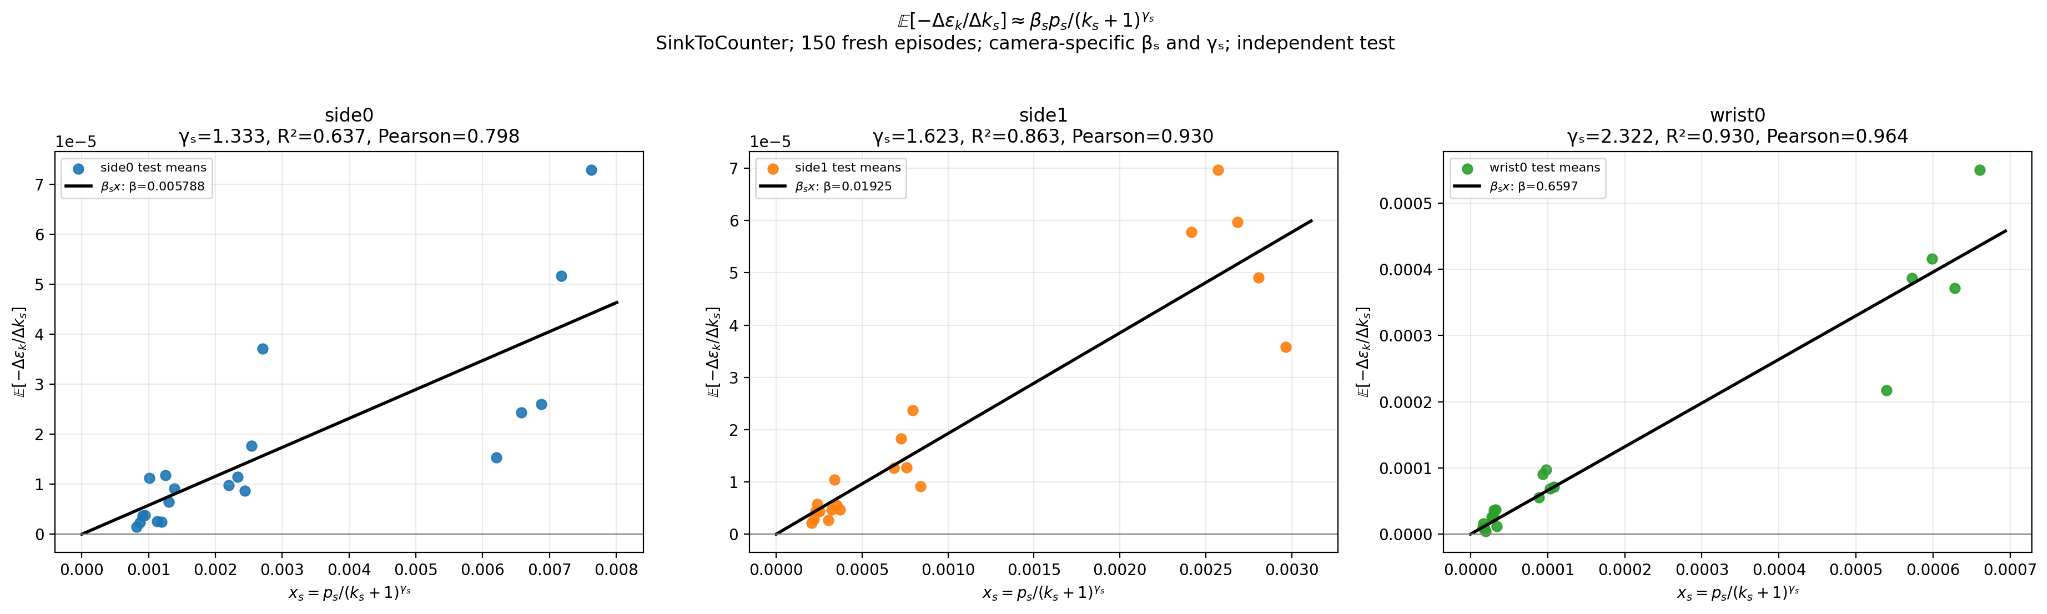
\includegraphics[width=0.98\textwidth]{marginal_utility_fit.png}
    \caption{Independent-test validation of the camera-specific marginal action utility law on SinkToCounter. The camera-specific $\beta_s$ and $\gamma_s$ are fitted on the calibration split and frozen before evaluation on 150 fresh episodes.}
    \label{fig:marginal_fit}
\end{figure*}
After calibration, $\beta_s^\star$ and $\gamma_s^\star$ are frozen and evaluated on fresh episodes that are not used for fitting. The validity of Lemma~\ref{lem:marginal_law} is assessed using the coefficient of determination $R^2$, Pearson correlation, Spearman rank correlation, and the residual error between the observed expected marginal gain and $\beta_s p_s/(k_s+1)^{\gamma_s}$. The resulting parameters are then stored as dataset-level constants and used by Algorithm~\ref{alg:allocation} throughout online execution.

\bibliographystyle{IEEEtranc}
\bibliography{IEEEfull, references} 

% \begin{thebibliography}{1}
% \bibliographystyle{IEEEtran}

% \bibitem{ref1}
% {\it{Mathematics Into Type}}. American Mathematical Society. [Online]. Available: https://www.ams.org/arc/styleguide/mit-2.pdf

% \bibitem{ref2}
% T. W. Chaundy, P. R. Barrett and C. Batey, {\it{The Printing of Mathematics}}. London, U.K., Oxford Univ. Press, 1954.

% \bibitem{ref3}
% F. Mittelbach and M. Goossens, {\it{The \LaTeX Companion}}, 2nd ed. Boston, MA, USA: Pearson, 2004.

% \bibitem{ref4}
% G. Gr\"atzer, {\it{More Math Into LaTeX}}, New York, NY, USA: Springer, 2007.

% \bibitem{ref5}M. Letourneau and J. W. Sharp, {\it{AMS-StyleGuide-online.pdf,}} American Mathematical Society, Providence, RI, USA, [Online]. Available: http://www.ams.org/arc/styleguide/index.html

% \bibitem{ref6}
% H. Sira-Ramirez, ``On the sliding mode control of nonlinear systems,'' \textit{Syst. Control Lett.}, vol. 19, pp. 303--312, 1992.

% \bibitem{ref7}
% A. Levant, ``Exact differentiation of signals with unbounded higher derivatives,''  in \textit{Proc. 45th IEEE Conf. Decis.
% Control}, San Diego, CA, USA, 2006, pp. 5585--5590. DOI: 10.1109/CDC.2006.377165.

% \bibitem{ref8}
% M. Fliess, C. Join, and H. Sira-Ramirez, ``Non-linear estimation is easy,'' \textit{Int. J. Model., Ident. Control}, vol. 4, no. 1, pp. 12--27, 2008.

% \bibitem{ref9}
% R. Ortega, A. Astolfi, G. Bastin, and H. Rodriguez, ``Stabilization of food-chain systems using a port-controlled Hamiltonian description,'' in \textit{Proc. Amer. Control Conf.}, Chicago, IL, USA,
% 2000, pp. 2245--2249.

% \end{thebibliography}


% \newpage

% \section{Biography Section}
% If you have an EPS/PDF photo (graphicx package needed), extra braces are
%  needed around the contents of the optional argument to biography to prevent
%  the LaTeX parser from getting confused when it sees the complicated
%  $\backslash${\tt{includegraphics}} command within an optional argument. (You can create
%  your own custom macro containing the $\backslash${\tt{includegraphics}} command to make things
%  simpler here.)
 
% \vspace{11pt}

% \bf{If you include a photo:}\vspace{-33pt}
% \begin{IEEEbiography}[{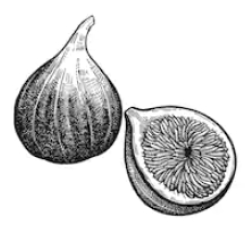
\includegraphics[width=1in,height=1.25in,clip,keepaspectratio]{fig1}}]{Michael Shell}
% Use $\backslash${\tt{begin\{IEEEbiography\}}} and then for the 1st argument use $\backslash${\tt{includegraphics}} to declare and link the author photo.
% Use the author name as the 3rd argument followed by the biography text.
% \end{IEEEbiography}

% \vspace{11pt}

% \bf{If you will not include a photo:}\vspace{-33pt}
% \begin{IEEEbiographynophoto}{John Doe}
% Use $\backslash${\tt{begin\{IEEEbiographynophoto\}}} and the author name as the argument followed by the biography text.
% \end{IEEEbiographynophoto}




\vfill

\end{document}


